\chapter{Protocolos Operativos de Gobernanza y Ética del Social Guide}
\label{anexo:protocolos-eticos}

Este anexo presenta los protocolos operativos para la gobernanza ética del \gls{social-guide}, complementando los fundamentos del Capítulo~\ref{chap:capitulo3}, Sección~\ref{sec:salvaguardas_eticas} y las directrices del Capítulo~\ref{chap:capitulo4}. Los principios aquí descritos no son sugerencias; son \textbf{condiciones necesarias}. Una organización que implementa \gls{socialscrum} sin estas salvaguardas convierte el marco en una herramienta de vigilancia, no de salud social~\cite{edmondson2018fearless, edmondson1999psychological}.

\section{Confidencialidad y protección de datos}

La confidencialidad es la base de la confianza del equipo en SocialScrum~\cite{mayer1995integrative}. El principio es absoluto:

\begin{quote}
    Toda información compartida en eventos sociales es \textbf{confidencial} y \textbf{no puede ser utilizada} para evaluaciones de desempeño, decisiones de contratación o despido, o cualquier acción que afecte el estatus laboral de un individuo.
\end{quote}

La única excepción es una obligación legal (investigación de acoso documentado), que requiere consentimiento explícito del afectado y documentación formal.

\subsection{Información confidencial vs. reportable}

La Tabla~\ref{tab:confidencial-reportable} de referencia rápida de información confidencial vs.\ reportable se presenta en la Sección~\ref{sec:salvaguardas_eticas} del Capítulo~\ref{chap:capitulo3}. A continuación se reproduce junto con los protocolos operativos detallados.

\begingroup
\scriptsize
\renewcommand{\arraystretch}{1.3}
\setlength{\tabcolsep}{4pt}
\setlength{\LTleft}{0pt}
\setlength{\LTright}{0pt}

\begin{longtable}{|
    >{\RaggedRight\hspace{0pt}}p{6.5cm}|
    >{\RaggedRight\hspace{0pt}}p{9cm}|
    }
    \caption{Información confidencial vs. reportable.} \label{tab:confidencial-reportable}                                 \\
    \hline
    \textbf{Confidencial (NO reportable)}        & \textbf{Reportable (datos agregados)}                                   \\
    \hline \endfirsthead
    \hline \endlastfoot
    Declaraciones individuales en retrospectivas & \gls{health-score} promedio del equipo                                  \\ \hline
    Conflictos interpersonales con nombres       & ``El equipo presenta aislamiento social'' (sin nombres)                 \\ \hline
    Estado emocional de personas específicas     & ``Se detectó \textit{burnout} en el equipo'' (sin identificar personas) \\ \hline
    Intención de renuncia de alguien             & ``Riesgo de rotación elevado'' (dato agregado)                          \\ \hline
    Críticas a gerencia por persona              & ``El equipo reporta fricción con \textit{stakeholders}''                \\ \hline
    Detalles de mediaciones 1:1                  & ``Se realizó mediación; conflicto en proceso de resolución''            \\
\end{longtable}
\endgroup

\noindent\textbf{Regla práctica:} si la información permite identificar a una persona y podría afectarla negativamente, es confidencial. Si describe al equipo sin señalar individuos, es reportable. El Anexo~\ref{anexo:confidencialidad} contiene la plantilla completa del Acuerdo de Confidencialidad del Social Guide, que formaliza: compromiso de no compartir información individual, reporte exclusivo de datos agregados, prohibición de uso para evaluaciones, rechazo de solicitudes de gerencia y remoción inmediata del rol ante violaciones.

\subsection{Protocolo técnico de protección de datos}

\begingroup
\scriptsize
\renewcommand{\arraystretch}{1.3}
\setlength{\tabcolsep}{4pt}
\setlength{\LTleft}{0pt}
\setlength{\LTright}{0pt}

\begin{longtable}{|
    >{\RaggedRight\hspace{0pt}}p{4cm}|
    >{\RaggedRight\hspace{0pt}}p{11.5cm}|
    }
    \caption{Requisitos técnicos de almacenamiento seguro.} \label{tab:almacenamiento-tecnico}                                                 \\
    \hline
    \textbf{Requisito}  & \textbf{Implementación}                                                                                              \\
    \hline \endfirsthead
    \hline \endlastfoot
    Cifrado en reposo   & AES-256 o equivalente; bases de datos con \textit{Transparent Data Encryption} (TDE).                                \\ \hline
    Cifrado en tránsito & HTTPS obligatorio; TLS~1.2 o superior.                                                                               \\ \hline
    Ubicación física    & Servidores en jurisdicciones con protección adecuada (GDPR si aplica); nunca en dispositivos personales sin cifrado. \\ \hline
    Separación lógica   & Base de datos separada de RR. HH. y de sistemas de evaluaciones de desempeño, sin acceso cruzado.                    \\
\end{longtable}
\endgroup

\subsubsection{Control de acceso}

\begingroup
\scriptsize
\renewcommand{\arraystretch}{1.3}
\setlength{\tabcolsep}{4pt}
\setlength{\LTleft}{0pt}
\setlength{\LTright}{0pt}

\begin{longtable}{|
    >{\RaggedRight\hspace{0pt}}p{4cm}|
    >{\RaggedRight\hspace{0pt}}p{11.5cm}|
    }
    \caption{Matriz de acceso a datos de SocialScrum.} \label{tab:matriz-acceso-socialscrum} \\
    \hline
    \textbf{Rol}       & \textbf{Acceso permitido}                                           \\
    \hline \endfirsthead
    \hline \endlastfoot
    Social Guide       & Acceso completo (lectura y escritura).                              \\ \hline
    Scrum Master       & Métricas agregadas (solo lectura).                                  \\ \hline
    CTO                & Métricas agregadas (solo lectura).                                  \\ \hline
    RR. HH. / Managers & Ninguno (acceso prohibido).                                         \\ \hline
    Auditor externo    & Solo lectura, limitado al periodo de auditoría.                     \\
\end{longtable}
\endgroup

\noindent Los accesos se implementan mediante roles técnicos en el sistema, no mediante confianza implícita.

\subsubsection{Retención y eliminación de datos}

\begin{description}[nosep, leftmargin=1.2cm, style=nextline]
    \item[Retención máxima] Datos individuales por 12 meses; después, solo agregados anonimizados.
    \item[Derecho de eliminación] Cualquier miembro puede solicitarla; el Social Guide tiene 5~días hábiles para ejecutarla.
    \item[Salida del equipo] Los datos individuales se eliminan en 30~días; los agregados permanecen.
    \item[Fin de SocialScrum] Todos los datos se eliminan en 60~días con notificación previa.
\end{description}

\noindent Toda consulta a datos debe generar un registro que indique el usuario, la marca de tiempo (\textit{timestamp}), los datos consultados y el origen. Los registros (\textit{logs}) se retienen 24~meses y se revisan mensualmente. Accesos anómalos generan una alerta automática.

\section{Estructura organizacional y rendición de cuentas}

La estructura organizacional del Social Guide y su justificación se presentan en el Capítulo~\ref{chap:capitulo3}, Sección~\ref{sec:salvaguardas_eticas}. La Figura~\ref{fig:estructura-sg} resume la cadena de reporte.

\begin{figure}[!htbp]
    \centering
    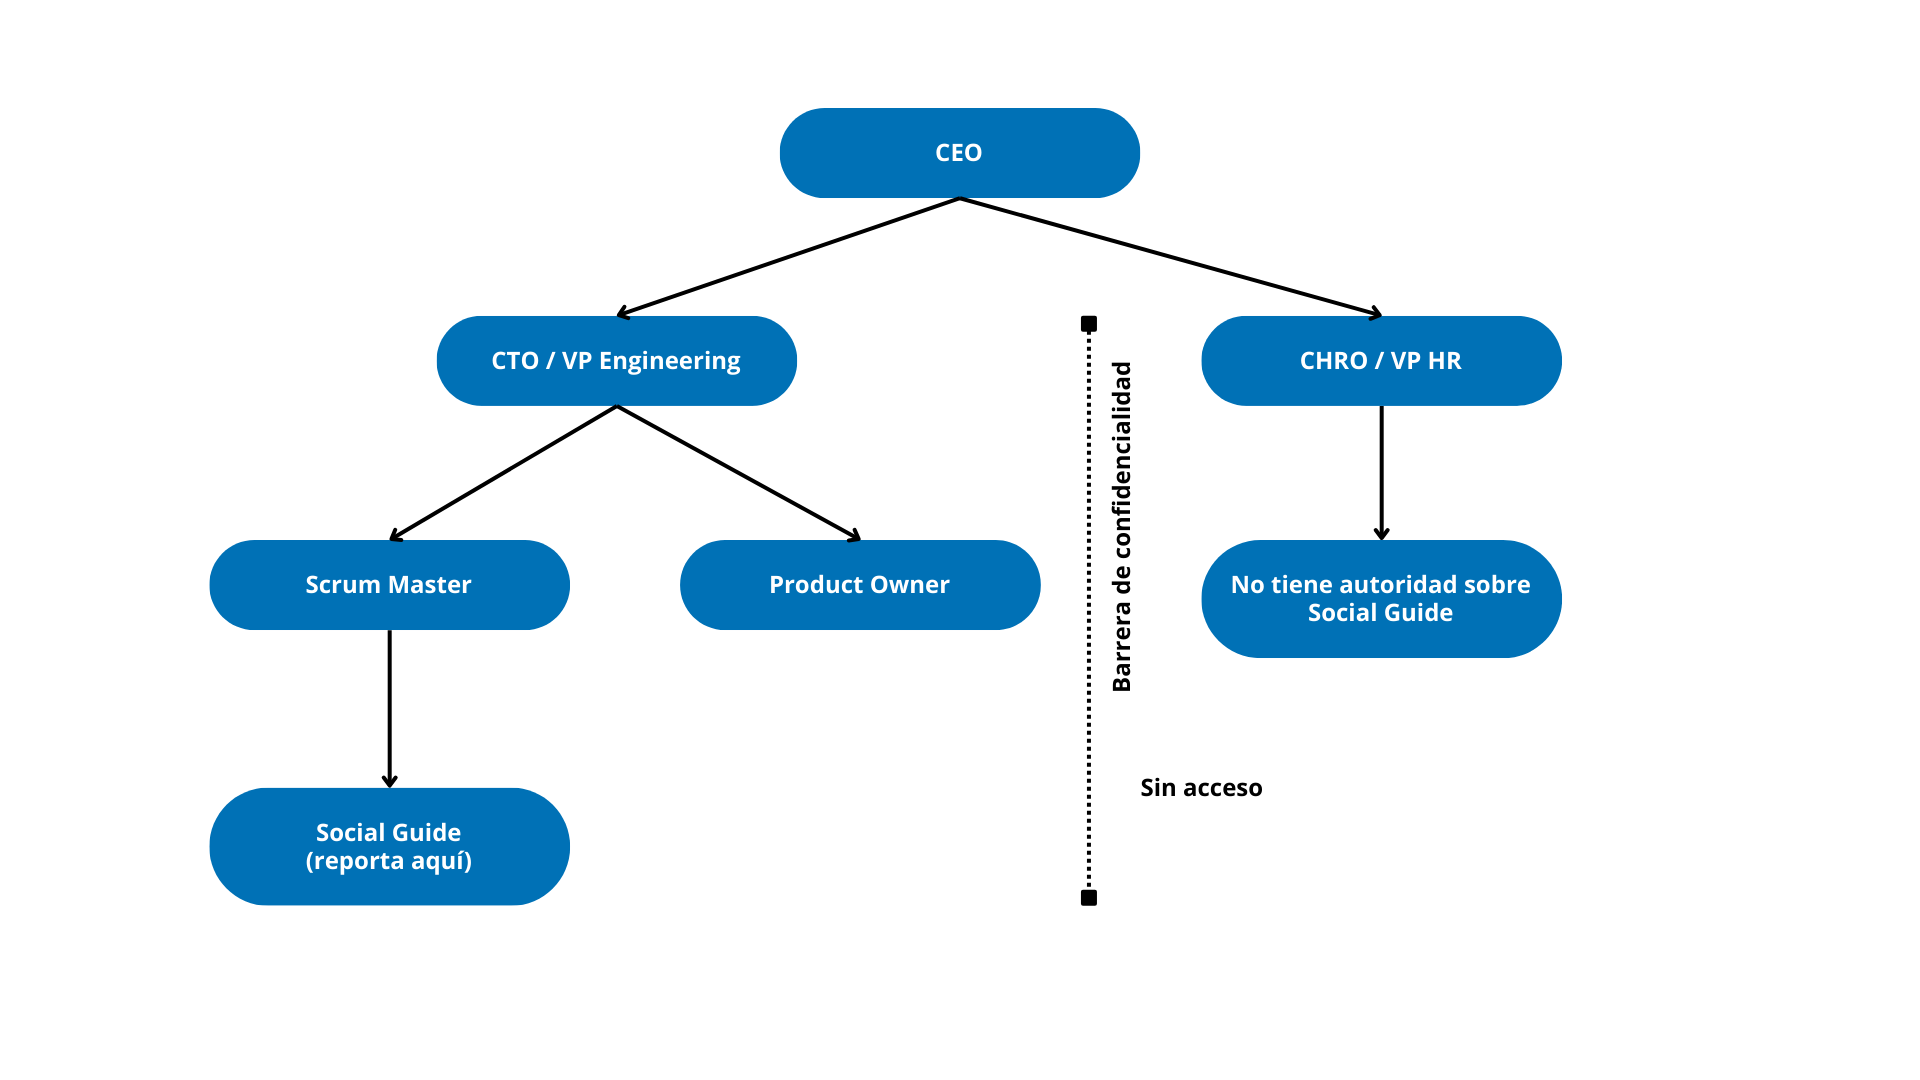
\includegraphics[width=0.7\textwidth]{recursos/capitulo4/estructura-sg.png}
    \caption{Estructura organizacional del Social Guide: reporta a CTO/SM, nunca a RR. HH.}
    \label{fig:estructura-sg}
\end{figure}
\FloatBarrier

Cuando RR. HH. solicita información individual, el Social Guide: (1)~rechaza inmediatamente, (2)~informa al SM/CTO, y (3)~documenta el intento. La organización debe establecer una política firmada por el CEO, el CTO y RR. HH. que prohíba el uso de datos de SocialScrum en evaluaciones de desempeño.

\section{Protocolo de conflicto PO--Social Guide}

Cuando el PO y el SG tienen visiones incompatibles sobre la priorización del Sprint y el diálogo no produce un acuerdo, se escala progresivamente:

\begin{enumerate}[nosep]
    \item \textbf{Nivel~1 -- Diálogo directo (30~min):} PO y SG exponen sus posiciones con datos y buscan un compromiso.
    \item \textbf{Nivel~2 -- Mediación del SM (1~hora):} El SM facilita una conversación estructurada; cada parte tiene 10~min sin interrupción.
    \item \textbf{Nivel~3 -- Decisión del CTO (24--48~h):} El SM presenta el caso por escrito; el CTO decide considerando el riesgo de negocio frente al riesgo social.
\end{enumerate}

\begin{figure}[!htbp]
    \centering
    \begin{tikzpicture}[scale=0.85]
        \node[rectangle, rounded corners, draw=blue!70, fill=blue!10, minimum width=2.5cm, minimum height=1.2cm, font=\footnotesize, align=center] (n1) at (0,2) {\textbf{Nivel 1}\\Diálogo directo\\{\tiny (30 min)}};
        \node[rectangle, rounded corners, draw=orange!70, fill=orange!10, minimum width=2.5cm, minimum height=1.2cm, font=\footnotesize, align=center] (n2) at (5,2) {\textbf{Nivel 2}\\Mediación SM\\{\tiny (1 hora)}};
        \node[rectangle, rounded corners, draw=red!70, fill=red!10, minimum width=2.5cm, minimum height=1.2cm, font=\footnotesize, align=center] (n3) at (10,2) {\textbf{Nivel 3}\\Decisión CTO\\{\tiny (24-48h)}};
        \node[rectangle, rounded corners, draw=green!70, fill=green!15, minimum width=2cm, minimum height=0.8cm, font=\footnotesize] (ok1) at (0,0) {Acuerdo};
        \node[rectangle, rounded corners, draw=green!70, fill=green!15, minimum width=2cm, minimum height=0.8cm, font=\footnotesize] (ok2) at (5,0) {Acuerdo};
        \node[rectangle, rounded corners, draw=green!70, fill=green!15, minimum width=2.2cm, minimum height=0.8cm, font=\footnotesize] (ok3) at (10,0) {Decisión final};
        \draw[-stealth, thick, red!60] (n1.east) -- (n2.west) node[midway, above, font=\tiny] {Sin acuerdo};
        \draw[-stealth, thick, red!60] (n2.east) -- (n3.west) node[midway, above, font=\tiny] {Sin acuerdo};
        \draw[-stealth, thick, green!60] (n1.south) -- (ok1.north) node[midway, right, font=\tiny] {Sí};
        \draw[-stealth, thick, green!60] (n2.south) -- (ok2.north) node[midway, right, font=\tiny] {Sí};
        \draw[-stealth, thick, green!60] (n3.south) -- (ok3.north);
        \node[font=\tiny, gray] at (0,3) {PO + SG};
        \node[font=\tiny, gray] at (5,3) {PO + SG + SM};
        \node[font=\tiny, gray] at (10,3) {CTO};
    \end{tikzpicture}
    \caption{Protocolo de escalamiento en conflicto PO--Social Guide}
    \label{fig:escalamiento-po-sg}
\end{figure}
\FloatBarrier

\subsection{Criterios de decisión para el CTO}

\begingroup
\scriptsize
\renewcommand{\arraystretch}{1.3}
\setlength{\tabcolsep}{4pt}
\setlength{\LTleft}{0pt}
\setlength{\LTright}{0pt}

\begin{longtable}{|
    >{\RaggedRight\hspace{0pt}}p{5.5cm}|
    >{\Centering\hspace{0pt}}p{4cm}|
    >{\RaggedRight\hspace{0pt}}p{5.5cm}|
    }
    \caption{Criterios de decisión en conflicto PO--SG.} \label{tab:criterios-conflicto}                                   \\
    \hline
    \textbf{Escenario}                      & \textbf{Recomendación}        & \textbf{Justificación}                       \\
    \hline \endfirsthead
    \hline \endlastfoot
    HS $>$ 7, \textit{deadline} contractual & Priorizar técnico             & Equipo sano puede absorber presión temporal. \\ \hline
    HS $<$ 4, \textit{deadline} flexible    & Priorizar social              & Equipo en crisis no entrega calidad.         \\ \hline
    HS 4--6, \textit{deadline} crítico      & Balance 50/50 o caso por caso & Zona gris; evaluar riesgo específico.        \\ \hline
    \gls{burnout} activo documentado        & Siempre priorizar social      & Ignorar \textit{burnout} garantiza rotación. \\
\end{longtable}
\endgroup

Si el mismo conflicto ocurre 3+ veces en 6~meses, indica un problema sistémico: si el PO siempre gana, revisar la autoridad formal del SG; si el SG siempre gana, revisar la comunicación con los \glspl{stakeholders}; si siempre escala al CTO, programar una sesión de alineación de roles.

\section{Protocolo de continuidad del Social Guide}

La salida del Social Guide (renuncia, despido, incapacidad) requiere proteger la continuidad del programa y la confidencialidad.

\subsection{Renuncia voluntaria (aviso $\geq$ 2 semanas)}

\begin{description}[nosep, leftmargin=1.2cm, style=nextline]
    \item[Semana~1] Notificación al SM, inicio del proceso de reemplazo y documentación del estado del equipo.
    \item[Semana~2] Entrenamiento del reemplazo (\textit{shadowing}), traspaso de documentación no individual y evento de cierre con el equipo.
    \item[Día final] Eliminación de accesos, destrucción o transferencia consentida de datos individuales y firma de compromiso de confidencialidad post-salida.
\end{description}

\subsection{Salida abrupta (despido, emergencia, incapacidad)}

\begin{description}[nosep, leftmargin=1.2cm, style=nextline]
    \item[Inmediato] El SM asume funciones mínimas; accesos revocados en $\leq 24$~h; el CTO autoriza acceso temporal del SM a la documentación agregada.
    \item[Semana~1] El SM revisa la documentación, identifica intervenciones urgentes y comunica la situación al equipo. Las notas individuales de sesiones 1:1 se destruyen si el SG no puede transferirlas con consentimiento.
    \item[Semanas 2--4] Selección acelerada del nuevo SG; el SM facilita solo los eventos básicos.
    \item[Nuevo SG] Inicia relaciones desde cero; recibe solo documentación agregada sobre \gls{community-smells} y el Health Score.
\end{description}

\noindent En ambos casos, el SG saliente firma un acuerdo de confidencialidad permanente (destrucción de notas personales, consecuencias legales por violaciones). El CTO actúa como testigo.

\section{Protocolo de auditoría independiente}

Cada 6~meses, un auditor independiente (externo, sin relación comercial, con experiencia en dinámicas de equipo) evalúa el cumplimiento ético del Social Guide.

\subsection{Proceso de auditoría}

\begin{enumerate}[nosep]
    \item \textbf{Entrevistas confidenciales} (30~min individuales, sin presencia del SG). Se evalúa (escala 1--10): percepción de confidencialidad, uso indebido de información, seguridad para ser auténtico, presión para compartir, conocimiento de derechos, observación de violaciones éticas y recomendación de SocialScrum.
    \item \textbf{Revisión de documentación:} reportes del SG, comunicaciones con gerencia/RR. HH., acuerdos firmados y evidencia de reportes no autorizados.
    \item \textbf{Reporte:} cumplimiento ético (Sí/No/Parcial), hallazgos, fortalezas y recomendaciones. El reporte es \textbf{público para el equipo}.
\end{enumerate}

\subsection{Consecuencias de hallazgos negativos}

Ante una posible violación ética identificada por el auditor, se inicia una investigación formal (CTO + auditor, 1--2~semanas). Si se \textbf{confirma la violación}: remoción inmediata del SG (sin posibilidad de retorno al rol), disculpa formal al equipo, nuevo SG con reentrenamiento ético, y auditoría de seguimiento a los 3~meses. Si \textbf{no se confirma pero hay preocupaciones}: \textit{feedback} detallado, plan de mejora, reauditoría a los 3~meses y monitoreo incrementado por el SM.

\subsection{Canal de denuncia y protección contra represalias}

Tres canales disponibles: (1)~interno (SM $\rightarrow$ CTO), (2)~externo (auditor independiente), (3)~anónimo (formulario web revisado por CTO + auditor). Política de tolerancia cero ante represalias: investigación inmediata, sanción al responsable (hasta despido), y protección formal del denunciante (12~meses de protección contra despido; evaluaciones negativas revisadas por auditor).

El Social Guide debe monitorear indicadores de represalias indirectas, tales como: asignación repentina de solo tareas triviales post-denuncia, exclusión de reuniones relevantes, aislamiento social por parte de colegas, calificaciones de desempeño inesperadamente bajas, oportunidades negadas o microgestión (\textit{micromanagement}) repentina. Ante un patrón sospechoso: (1)~documentar con fechas, (2)~entrevistar confidencialmente al afectado, (3)~si confirma represalia, escalar a CTO, (4)~si no, documentar y revisar en 30~días.

\section{Prevención del ``Teatro Social''}

El ``Teatro Social'' ocurre cuando el equipo simula bienestar mientras los problemas reales permanecen ocultos.

\subsection{Síntomas y causas}

\begingroup
\scriptsize
\renewcommand{\arraystretch}{1.3}
\setlength{\tabcolsep}{4pt}
\setlength{\LTleft}{0pt}
\setlength{\LTright}{0pt}

\begin{longtable}{|
    >{\RaggedRight\hspace{0pt}}p{4.5cm}|
    >{\RaggedRight\hspace{0pt}}p{10.8cm}|
    }
    \caption{Síntomas del ``Teatro Social''.} \label{tab:sintomas-teatro}                                \\
    \hline
    \textbf{Síntoma}             & \textbf{Descripción}                                                  \\
    \hline \endfirsthead
    \hline \endlastfoot
    HS artificialmente alto      & Valores entre 8--10 sin variación, incluso con problemas visibles.    \\ \hline
    Retrospectivas sin sustancia & ``Todo bien'', ``sin comentarios''; ausencia de crítica constructiva. \\ \hline
    Discrepancia con la realidad & HS de 9/10 mientras la velocidad cae o hay rotación elevada.          \\ \hline
    Participación forzada        & Respuestas rápidas sin reflexión real.                                \\ \hline
    Miedo a ser diferentes       & Nadie puntúa bajo porque ``todos puntúan alto''.                      \\
\end{longtable}
\endgroup

Las causas principales son: (1)~\textbf{miedo a represalias} (historial de información usada contra personas, SG cercano a gerencia, cultura de ``matar al mensajero''); (2)~\textbf{presión por buenos números} (HS tratado como KPI de vanidad); (3)~\textbf{fatiga de retrospectiva} (percepción de burocracia sin impacto); (4)~\textbf{SG inefectivo} (no genera confianza o es percibido como ``espía de gerencia'').

\subsection{Estrategias de prevención}

\paragraph{Estrategia~1: Nunca premiar o castigar por Health Score.} El HS es un instrumento diagnóstico, no un KPI. Está \textbf{prohibido} celebrar HS altos, asociar bonos o incentivos, o presionar para ``mejorar el número''. Está \textbf{permitido} usarlo como señal de necesidad de apoyo y para asignar recursos de intervención social.

\paragraph{Estrategia~2: Validación cruzada de datos.}

\begingroup
\scriptsize
\renewcommand{\arraystretch}{1.3}
\setlength{\tabcolsep}{4pt}
\setlength{\LTleft}{0pt}
\setlength{\LTright}{0pt}

\begin{longtable}{|
    >{\RaggedRight\hspace{0pt}}p{3.5cm}|
    >{\RaggedRight\hspace{0pt}}p{4.5cm}|
    >{\RaggedRight\hspace{0pt}}p{7cm}|
    }
    \caption{Validación cruzada del Health Score.} \label{tab:validacion-cruzada}                          \\
    \hline
    \textbf{Health Score} & \textbf{Indicador objetivo}   & \textbf{Interpretación}                        \\
    \hline \endfirsthead
    \hline \endlastfoot
    Alto (8+)             & Velocidad estable o creciente & Consistente: probablemente real.               \\ \hline
    Alto (8+)             & Velocidad cayendo             & Inconsistente: posible ``Teatro Social''.      \\ \hline
    Alto (8+)             & Rotación reciente             & Inconsistente: requiere investigación.         \\ \hline
    Bajo ($<$4)           & Velocidad baja                & Consistente: el equipo está siendo honesto.    \\ \hline
    Bajo ($<$4)           & Velocidad alta                & Inusual: equipo muy crítico o problema oculto. \\
\end{longtable}
\endgroup

\paragraph{Estrategia~3: Encuestas anónimas de validación.} Cada 2--3 Sprints, una encuesta completamente anónima con 4~preguntas: (1)~¿El HS refleja la realidad? (Sí / Parcialmente / No), (2)~¿Te sientes seguro para ser honesto? (Sí / Parcialmente / No, temo consecuencias), (3)~¿Hay algo que el equipo no dice pero debería? (respuesta abierta), (4)~¿Confías en la confidencialidad del SG? (Sí / No estoy seguro / No). Si revela discrepancias significativas, investigar causas y potencialmente reiniciar la construcción de confianza.

\paragraph{Estrategia~4: Rotación del facilitador de retrospectiva.} Rotar con el SM o miembros voluntarios puede revelar dinámicas que el SG, como facilitador habitual, no capta.

\paragraph{Estrategia~5: Celebrar la honestidad, no los números.} La comunicación correcta es: ``Prefiero un Health Score de 5 real que un 9 ficticio''. La comunicación incorrecta (tipo KPI) es: ``Felicitaciones, su HS subió de 6 a 8''.

\subsection{Protocolo ante detección de ``Teatro Social''}

Se activa cuando: la encuesta anónima revela desconfianza ($>30~\%$ ``No me siento seguro''), hay un HS alto con métricas técnicas inconsistentes, o hay retrospectivas sin sustancia durante 3+ Sprints. Las acciones son:

\begin{enumerate}[nosep]
    \item \textbf{No confrontar al equipo} (la confrontación destruye la confianza restante).
    \item \textbf{Reflexión del SG:} ¿qué comportamientos propios generan desconfianza? ¿Hay incentivos estructurales perversos?
    \item \textbf{Sesión de reinicio} facilitada por un actor externo: reconocer que algo no funciona, preguntar ``¿Qué necesitan para ser honestos?'' y escuchar sin justificar.
    \item \textbf{Ajustes estructurales:} reforzar garantías de confidencialidad, considerar el cambio de SG si la confianza es irrecuperable, verificar presiones de gerencia.
    \item \textbf{Período de reconstrucción} (3--6 Sprints): aceptar HS bajos pero realistas, enfatizar acciones sobre métricas, reforzar señales de honestidad emergente.
\end{enumerate}

\medskip

Las salvaguardas éticas son condición necesaria para que SocialScrum funcione. Sin confidencialidad, el equipo no será auténtico. Sin la estructura organizacional correcta, la información se usará mal. Sin auditoría, no hay verificación. Sin prevención del ``Teatro Social'', el Health Score será una métrica de vanidad. La regla de oro: si hay duda sobre si algo es ético, no se hace.